\documentclass[11pt,a4paper]{article}
\usepackage[T1]{fontenc}
\usepackage[utf8]{inputenc}
\usepackage[polish]{babel}
\usepackage{lmodern}
\usepackage[a4paper,margin=2.5cm]{geometry}
\usepackage{graphicx}
\usepackage{booktabs}
\usepackage{amsmath}
\usepackage{xcolor}
\usepackage{listings}
\usepackage{caption}
\usepackage{float}
\usepackage[colorlinks=true,linkcolor=blue!40!black,urlcolor=blue!40!black,citecolor=blue!40!black]{hyperref}

\definecolor{kwcol}{RGB}{40,70,130}
\definecolor{cmcol}{RGB}{90,110,90}
\definecolor{numcol}{RGB}{120,120,120}
\lstset{
  language=C++, basicstyle=\ttfamily\footnotesize, keywordstyle=\color{kwcol},
  commentstyle=\color{cmcol}\itshape, numbers=left, numberstyle=\tiny\color{numcol},
  numbersep=6pt, frame=single, rulecolor=\color{black!25}, breaklines=true,
  columns=fullflexible, keepspaces=true, xleftmargin=1.5em, framexleftmargin=1.5em,
  morekeywords={omp, pragma, parallel, schedule, reduction, critical, atomic, for}
}
\captionsetup{font=small,labelfont=bf}
\captionsetup[table]{position=above}
\captionsetup[figure]{position=below}

\title{Laboratorium 2: OpenMP\\\large Równoległa analiza chmury punktów}
\author{Jakub Balicki}
\date{listopad 2026}

\begin{document}
\maketitle
\vspace{-1em}

\section{Zadanie i implementacja}
Program wczytuje chmurę 6\,865\,878 punktów XYZ i dla każdego liczy kąt $\alpha=\mathrm{atan2}(y-Y_0,x-X_0)$, promień $r=\sqrt{dx^2+dy^2}$ oraz $\mathrm{value}=\sin\alpha\cos\alpha\,\ln(r+1)$, gdzie $X_0=566809{,}6$, $Y_0=243450{,}1$. Następnie wyznacza $\min$, $\max$ i sumę \texttt{value} oraz histogram liczby punktów w 100 sektorach kątowych po $3{,}6^\circ$. Statystyki liczone są klauzulą \texttt{reduction}. Problemem jest histogram, bo wiele wątków zwiększa te same komórki, więc porównano trzy sposoby synchronizacji:
\begin{lstlisting}
#pragma omp critical            // 1) cala inkrementacja w sekcji krytycznej
{ hist[s]++; }
#pragma omp atomic              // 2) atomowa inkrementacja komorki
hist[s]++;
// 3) prywatny histogram w kazdym watku, scalany raz na koniec
#pragma omp critical
{ for (int k=0;k<NSECT;++k) hist[k]+=local[k]; }
\end{lstlisting}
Wszystkie trzy wersje dają histogram identyczny z sekwencyjnym; statystyki: $\min=-3{,}004412$, $\max=2{,}999249$, $\sum=-1\,597\,174{,}73$.

Pomiary: AMD Ryzen 7 5700X (8 rdzeni, 16 wątków sprzętowych), g++ 15.2.0 z flagami \texttt{-O3 -fopenmp}. Podano medianę z 7 powtórzeń czasu samej analizy (\texttt{omp\_get\_wtime()}); baza to osobna wersja sekwencyjna, $T_{\mathrm{seq}}=214{,}0$\,ms.

\section{Wyniki}
Rozkład punktów w sektorach jest nierówny (rys.~\ref{fig:hist}): od 3\,919 punktów w sektorze 53 do 158\,386 w sektorze 87. To cecha danych i nie wpływa na analizę skalowania.

\begin{figure}[H]
\centering
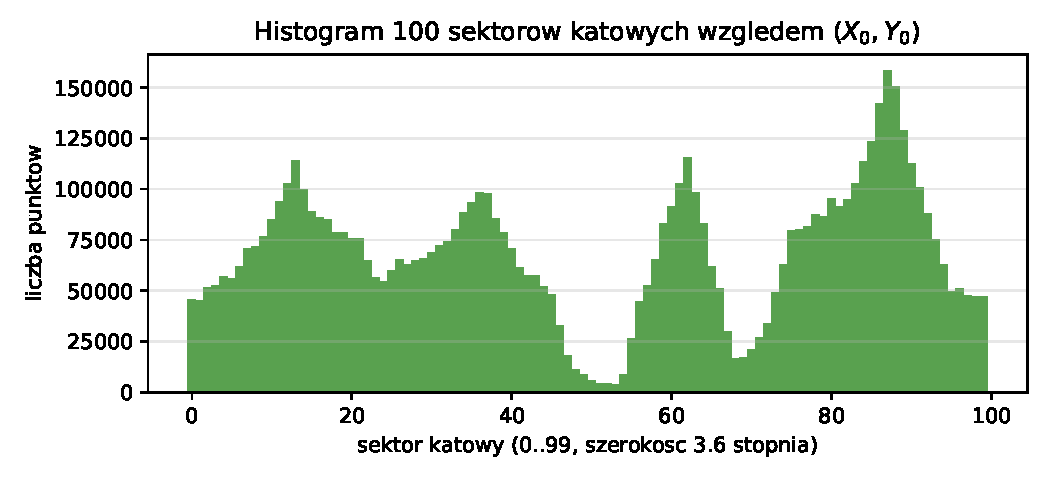
\includegraphics[width=0.8\textwidth]{histogram.pdf}
\caption{Histogram 100 sektorów kątowych.}\label{fig:hist}
\end{figure}

\begin{table}[H]
\centering
\caption{Mediana czasu [ms] i przyspieszenie $S_p=T_{\mathrm{seq}}/T_p$ (w nawiasie) dla trzech metod histogramu.}\label{tab:sync}
\small\setlength{\tabcolsep}{4pt}\begin{tabular}{lccccc}
\toprule
Metoda & $p=1$ & $p=2$ & $p=4$ & $p=8$ & $p=16$ \\
\midrule
\texttt{critical}         & 233,3 (0,92) & 272,9 (0,78) & 559,7 (0,38) & 979,6 (0,22) & 1274,8 (0,17) \\
\texttt{atomic}           & 219,5 (0,98) & 120,5 (1,78) & 64,9 (3,30) & 36,9 (5,80) & 31,6 (6,77) \\
prywatne histogramy       & 211,2 (1,01) & 107,0 (2,00) & 57,5 (3,72) & 31,9 (6,71) & 32,3 (6,64) \\
\bottomrule
\end{tabular}
\end{table}

\begin{figure}[H]
\centering
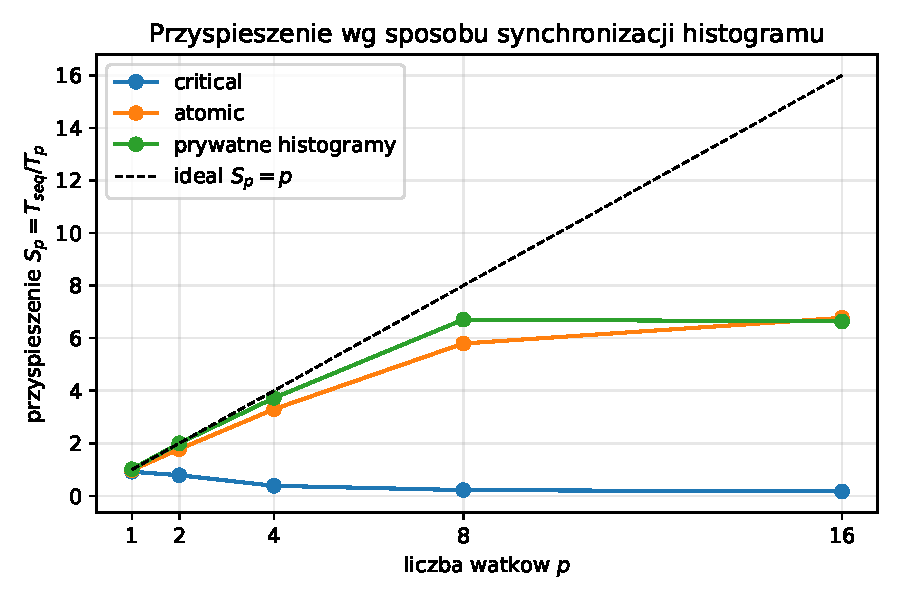
\includegraphics[width=0.55\textwidth]{speedup.pdf}
\caption{Przyspieszenie względem wersji sekwencyjnej; linia przerywana to ideał $S_p=p$.}\label{fig:speedup}
\end{figure}

\begin{figure}[H]
\centering
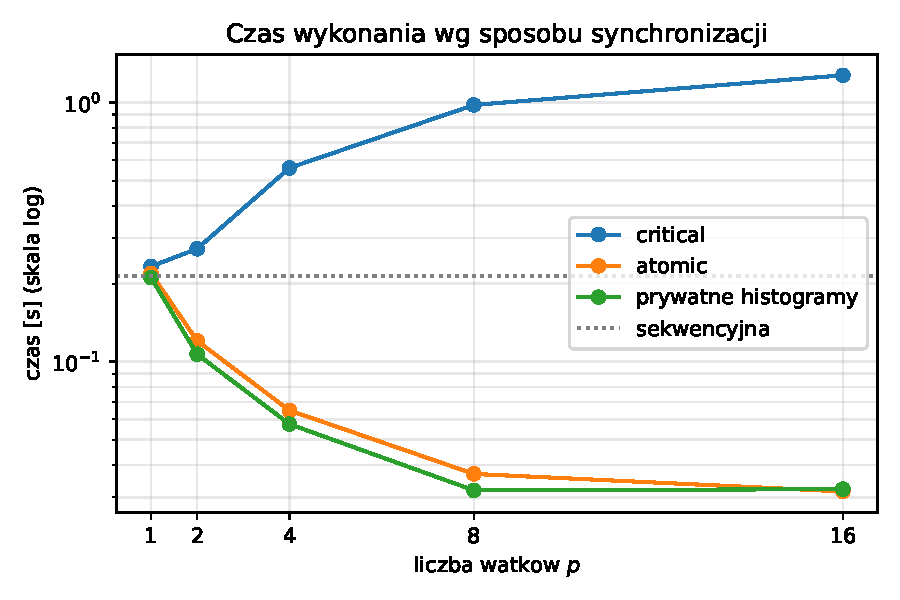
\includegraphics[width=0.55\textwidth]{synchronizacja.pdf}
\caption{Czas wykonania (skala logarytmiczna); \texttt{critical} rośnie z liczbą wątków.}\label{fig:sync}
\end{figure}

Dla prywatnych histogramów i 16 wątków porównano też strategie \texttt{schedule} (mediana, ms): \texttt{static} 32,25, \texttt{static,1000} 31,79, \texttt{static,100000} 35,07, \texttt{dynamic,1000} 28,79, \texttt{dynamic,100000} 30,21, \texttt{guided} 30,10.

\begin{figure}[H]
\centering
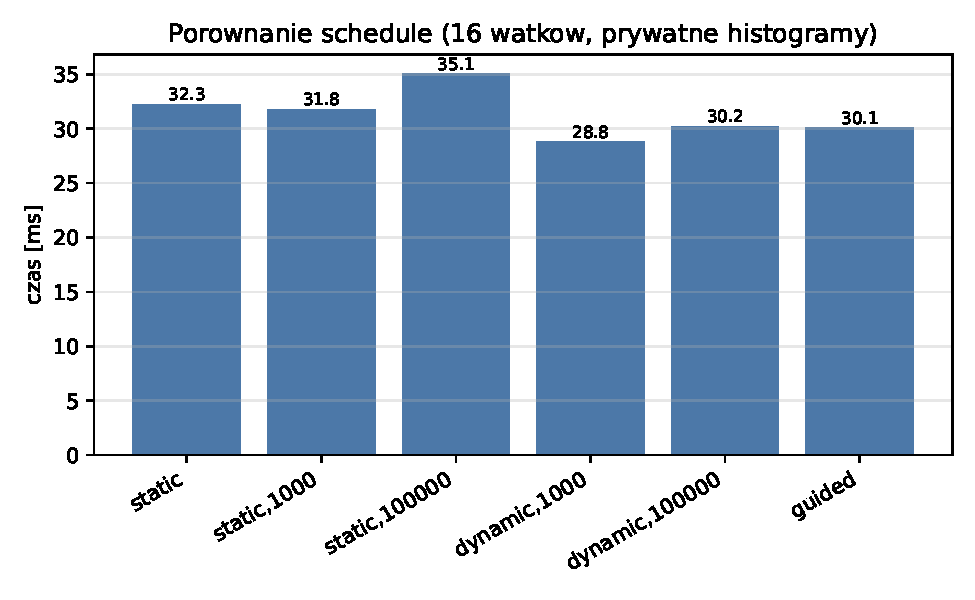
\includegraphics[width=0.55\textwidth]{schedule.pdf}
\caption{Czas dla różnych strategii \texttt{schedule} (16 wątków).}\label{fig:sched}
\end{figure}

\section{Wnioski}
\begin{itemize}
\item \texttt{critical} serializuje każdą inkrementację, więc czas rośnie z liczbą wątków (z 233\,ms do 1275\,ms przy 16) i zrównoleglenie tylko szkodzi.
\item \texttt{atomic} skaluje się dobrze ($S_{16}=6{,}77$), a prywatne histogramy są najlepsze ($S_8=6{,}71$), bo synchronizacja zachodzi raz na wątek, a nie raz na punkt.
\item Powyżej 8 wątków (liczba rdzeni fizycznych) przyspieszenie przestaje rosnąć.
\item Wybór \texttt{schedule} ma niewielki wpływ; najkrótszy czas dało \texttt{dynamic,1000} (28,8\,ms), ale różnice mieszczą się w rozrzucie pomiarów.
\end{itemize}

\end{document}
